\documentclass[10pt]{beamer}
\usepackage[utf8]{inputenc}
\usepackage[T1]{fontenc}
\usepackage[portuguese]{babel}
\usepackage{amsmath}
\usepackage{amsfonts}
\usepackage{amssymb}
\usepackage{graphicx}
\usetheme{Madrid}
\usepackage{multicol}
\begin{document}
	\author{António Fróis}
	\title{Apresentação em Beamer}
	\subtitle{Laboratório Zorex}
	\logo{
\includegraphics[scale=0.1]{Fcul.png}}
	\institute{Faculdade de Ciências}
	\date{01 de Dezembro de 2017}
	\subject{Produção de Documentos Técnicos}
	%\setbeamercovered{transparent}
	%\setbeamertemplate{navigation symbols}{}
	\begin{frame}[plain]
	\maketitle
\end{frame}

\begin{frame}
\frametitle{Tabela otimizada \\ Nº de Funcionários = 435}
\begin{table}
\label{T2}
\resizebox{\columnwidth}{2,5cm}{
\begin{tabular}{ | c | c | c | c | c | c | c | c | c | c | c | c | c | }
\hline
	\multicolumn{1}{|c|}{Dia} & \multicolumn{1}{c|}{\begin{tabular}[c]{@{}c@{}}Nº\\ Aleatório\end{tabular}} & \multicolumn{1}{c|}{\begin{tabular}[c]{@{}c@{}}Nº de\\  Encomendas\\ Recebidas\end{tabular}} & \multicolumn{1}{c|}{\begin{tabular}[c]{@{}c@{}}Nºde\\  Encomendas\\ a Produzir\end{tabular}} & \multicolumn{1}{c|}{\begin{tabular}[c]{@{}c@{}}Capacidade \\ de \\ Produção Diária\end{tabular}} & \multicolumn{1}{c|}{\begin{tabular}[c]{@{}c@{}}Nº de \\ Encomendas\\ Produzidas\end{tabular}} & \multicolumn{1}{c|}{\begin{tabular}[c]{@{}c@{}}Nº de \\ Encomendas\\ em Atraso\end{tabular}} & \multicolumn{1}{c|}{\begin{tabular}[c]{@{}c@{}}Percentagem da \\ Ocupação\\ da mão-de-obra\end{tabular}} \\ \hline
	1 & 0.49 & 60000 & 60000 & 65685 & 65685 & 0 & 1 \\ \hline
	2 & 0.94 & 70000 & 70000 & 65685 & 65685 & 4315 & 1 \\ \hline
	3 & 0.69 & 65000 & 69315 & 65685 & 65685 & 3630 & 1  \\ \hline
	4 & 0.7 & 65000 & 68630 & 65685 & 65685 & 2945 & 1  \\ \hline
	5 & 0.47 & 60000 & 62945 & 65685 & 62945 & 0 & 0.95828575778336 \\ \hline
	6 & 0.76 & 65000 & 65000 & 65685 & 65000 & 0 & 0.98957143944584003  \\ \hline
	7 & 0.86 & 65000 & 65000 & 65685 & 65000 & 0 & 0.98957143944584003  \\ \hline
	8 & 0.4 & 60000 & 60000 & 65685 & 60000 & 0 & 0.91345055948846765  \\ \hline
	9 & 0.63 & 65000 & 65000 & 65685 & 65000 & 0 & 0.98957143944584003  \\ \hline
	10 & 0.19 & 55000 & 55000 & 65685 & 55000 & 0 & 0.83732967953109538 \\ \hline
	11 & 0.5 & 60000 & 60000 & 65685 & 60000 & 0 & 0.91345055948846765  \\ \hline
	12 & 0.54 & 60000 & 60000 & 65685 & 60000 & 0 & 0.91345055948846765  \\ \hline
	13 & 0.37 & 60000 & 60000 & 65685 & 60000 & 0 & 0.91345055948846765  \\ \hline
	14 & 0.54 & 60000 & 60000 & 65685 & 60000 & 0 & 0.91345055948846765  \\ \hline
	15 & 0.76 & 65000 & 65000 & 65685 & 65000 & 0 & 0.98957143944584003  \\ \hline
	16 & 0.08 & 50000 & 50000 & 65685 & 50000 & 0 & 0.76120879957372312  \\ \hline
	17 & 0.41 & 60000 & 60000 & 65685 & 60000 & 0 & 0.91345055948846765  \\ \hline
	18 & 0.36 & 60000 & 60000 & 65685 & 60000 & 0 & 0.91345055948846765  \\ \hline
	19 & 0.13 & 50000 & 50000 & 65685 & 50000 & 0 & 0.76120879957372312  \\ \hline
	20 & 0.8 & 65000 & 65000 & 65685 & 65000 & 0 & 0.98957143944584003  \\ \hline
	21 & 0.25 & 55000 & 55000 & 65685 & 55000 & 0 & 0.83732967953109538  \\ \hline
	22 & 0.78 & 65000 & 65000 & 65685 & 65000 & 0 & 0.98957143944584003  \\ \hline
	23 & 0.76 & 65000 & 65000 & 65685 & 65000 & 0 & 0.98957143944584003  \\ \hline
	24 & 0.77 & 65000 & 65000 & 65685 & 65000 & 0 & 0.98957143944584003  \\ \hline
	25 & 0.76 & 65000 & 65000 & 65685 & 65000 & 0 & 0.98957143944584003  \\ \hline
	26 & 0.59 & 60000 & 60000 & 65685 & 60000 & 0 & 0.91345055948846765  \\ \hline
	27 & 0.4 & 60000 & 60000 & 65685 & 60000 & 0 & 0.91345055948846765  \\ \hline
	28 & 0.05 & 50000 & 50000 & 65685 & 50000 & 0 & 0.76120879957372312  \\ \hline
	29 & 0.02 & 50000 & 50000 & 65685 & 50000 & 0 & 0.76120879957372312 \\ \hline
	30 & 0.63 & 65000 & 65000 & 65685 & 65000 & 0 & 0.98957143944584003 \\ \hline
\end{tabular}}
\caption{Tabela otimizada do caso onde se contratam 435 trabalhadores}
\end{table}
\end{frame}

\begin{frame}
\frametitle{Gráfico}
\begin{figure}[h]	\label{G1} 
\begin{center}
	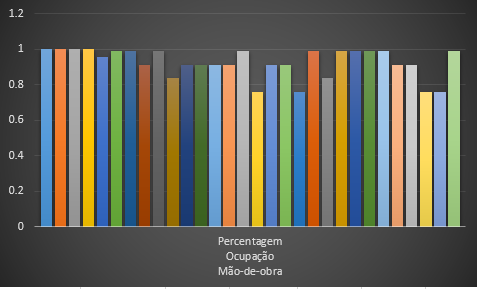
\includegraphics[scale=0.5]{GOtimizado.PNG}
	\caption{Gráfico Otimizado da Percentagem da Ocupação da mão-de-obra}
\end{center}
\end{figure}
\end{frame}

\begin{frame}
\frametitle{Princípios usados para a otimização}
\begin{enumerate}
\item Percentagem de Ocupação da mão-de-obra deve ser acima de 90\%
\item Número de encomendas em atraso deve ser inferior a 500
\item Encontrar um equilibrio entre a percentagem da ocupação da mão-de-obra e o número de encomendas em atraso 
\end{enumerate}
\end{frame}

\begin{frame}
\begin{figure}\footnote{Imagem retirada de http://medicodental-club.blogspot.pt/2011/07/local-anesthesia.html}
	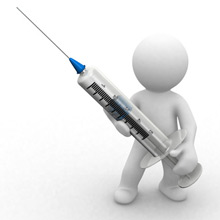
\includegraphics[scale=0.5]{F1.png}
\end{figure}
\end{frame}

\end{document}